%This work is licensed under the Creative Commons Attribution-NonCommercial-NoDerivs 3.0 United States License. To view a copy of this license, visit http://creativecommons.org/licenses/by-nc-nd/3.0/us/ or send a letter to Creative Commons, 444 Castro Street, Suite 900, Mountain View, California, 94041, USA.

% the content of this section is a modification of our APL paper on ESTE

%Sub-nanosecond (ultrafast) pulsed laser-driven electron sources are now being employed in a wide variety of scientific studies: in particular, ultrafast electron diffraction (UED)\cite{sciaini_femtosecond_2011}, ultrafast transmission electron microscopy (UEM)\cite{king_ultrafast_2005}, and pulsed X-ray free electron lasers\cite{dowell_cathode_2010}.
The spatial quality of the sources for UEM and UED are often characterized in terms of their normalized transverse rms emittance\cite{dowell_quantum_2009,jensen_emittance_2010}; $\varepsilon_{\smallT} = \Delta p_x \Delta x / (m_0 c)$, where $\Delta p_x = \sqrt{ \langle p_x^2 \rangle }$ is the rms transverse momentum of the source and $\Delta x = \sqrt{ \langle x^2 \rangle }$  is its size (cylindrical symmetry assumed), and $m_0$ is the electron rest mass and $c$ is the speed of light in vacuum.
As a reduction in the source size $\Delta x$ is limited either by the attainable diffraction-limited focusing or by the short-pulse Child's Law (screening of the electron gun's acceleration field)\cite{valfells_effects_2002}, significant improvements in the performance of scientific instruments employing pulsed electron sources through a reduction in their spatial emittance $\varepsilon_{\smallT}$ (and consequent increase in brightness\cite{berger_dc_2009}) may only be possible by decreasing the rms transverse momentum $\Delta p_x$ of the electron source --- an intrinsic property of the emission source\cite{dowell_quantum_2009,jensen_emittance_2010}.  

\section{Experimental Methodology} \label{sec:photocathode-method}

\begin{figure}
  \centering
  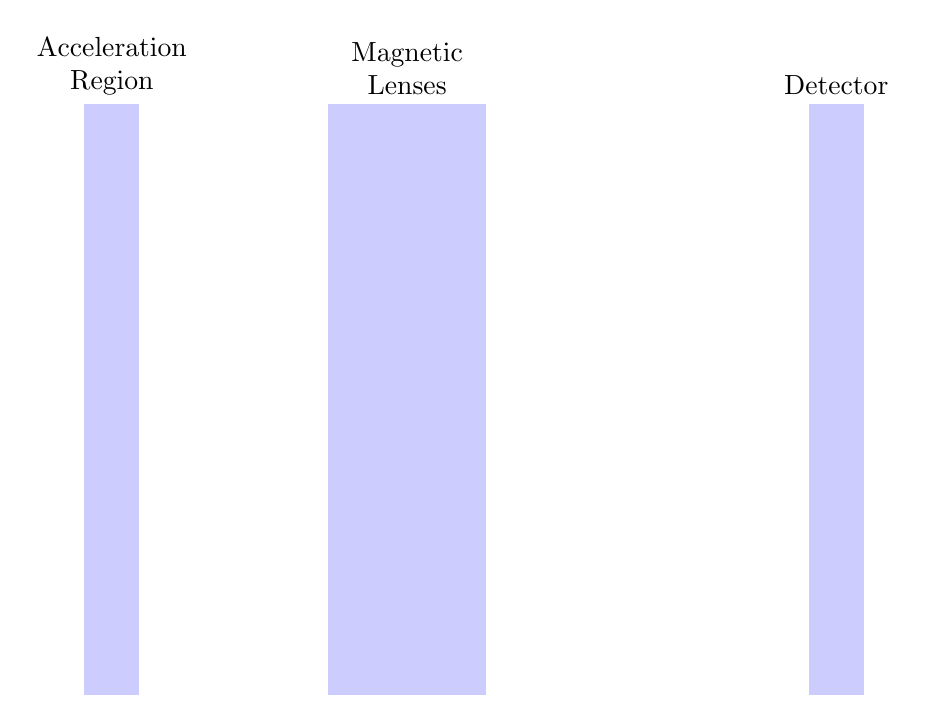
\begin{tikzpicture}
  \fill [blue!20] 
    (1.3,0.95)
    -- ++(0.7,0)
    -- ++(0,7.5)
    -- ++(-0.7,0)
      node [black, above, pos=0.5, align=center] {Acceleration\\Region}
    -- cycle
  ;
  \fill [blue!20]
    (4.4,0.95)
    -- ++(2,0)
    -- ++(0,7.5)
    -- ++(-2,0)
      node [black, pos=0.5, above, align=center] {Magnetic\\Lenses}
    -- cycle
  ;
  \fill [blue!20] 
    (10.5,0.95)
    -- ++(0.7,0)
    -- ++(0,7.5)
    -- ++(-0.7,0)
      node [black, above, pos=0.5] {Detector}
    -- cycle
  ;
  \inputdata{fig1data}
\end{tikzpicture}

  \caption{
    Simulations of the electron pulse propagation through the apparatus using the extended AG model.  
    Solid line: The spatial beam width (normalized to that at the photocathode $\Delta x_0$) with the magnetic lens strengths adjusted to ensure that the detector is at their back focal plane (Fourier plane).
    Dashed line: The case when the strength of the magnetic lenses is increased by a factor of two to focus the electron beam on the YAG scintillator detector.
  }
  \label{fig:transverse-measurement}
\end{figure}

\ref{fig:transverse-measurement} depicts the experimental technique used to determine directly the transverse momentum distributions (and hence $\Delta p_x$) of the laser-driven electron sources.
The primary laser radiation source for the studies is a home-built, diode-pumped and thermal-lens-shaped, femtosecond Yb:KGW oscillator\cite{berger_high-power_2008} delivering 250fs duration pulses at 1047nm and a 63MHz repetition rate (see Section \ref{sec:laser}).
This 2W average power laser is frequency doubled in a 3mm lithium triborate (LBO) crystal with 50\% efficiency to yield $\sim$200fs green pulses at 523nm (photon energy, $\hbar \omega$ = 2.37eV) (see Section \ref{sec:laser}).
Further doubling with a cylindrical focusing geometry in a 7mm $\beta$-barium borate (BBO) crystal yields 261nm ($\hbar \omega$ = 4.75eV) UV pulses with a duration of $\sim$4ps (due to the 600fs/mm group velocity mismatch between the green and generated UV).
Both the green and UV laser pulses are focused with 30cm focal lenses onto the photocathode in a 20kV electron gun at an angle of incidence of $60(\pm5)^{\circ}$, which improves the coupling of the $p$-polarized laser radiation into the photocathode surface\cite{berger_dc_2009}.
The electron gun design is based on the that of Togawa et al.\cite{berger_dc_2009,togawa_ceb6_2007} and has an acceleration gap of 25($\pm$2)mm.
After acceleration in the DC photo-gun, the electrons pass through a set of electrostatic deflection plates to ensure that the electron beam passes, as close as possible, axially through the center of two, 6.35mm-bore, thin and round magnetic lenses with counter-propagating currents to minimize image rotation effects.
A YAG scintillator placed 27.5cm after the second magnetic lens detects the spatial electron beam profile, and its visible fluorescence is 1:1 imaged onto a CCD detector with 5.4$\mu$m pixels. 
%TODO internal cross-references to appropriate sections above

To ensure that the transverse momentum distribution is observed, the YAG scintillator must be positioned at the back focal plane (the Fourier plane) of the lens system.
This is readily achieved by appropriate adjustment of the current $I$ in the magnetic lens coils; specifically, after determining the current required to focus the electron beam onto the scintillator, optical imaging relations together with the $I^2$ dependence of the magnetic lens strength are used to find the current that ensures that the average lens to scintillator distance equals the focal length of the lens system.
Simulation of the experimental apparatus (employing the extended AG model, see Section \ref{sec:external_forces} ), also shown in \ref{fig:transverse-measurement}, confirms that this procedure places the YAG scintillator at the back focal plane of the lens system to within a $\pm$0.5cm error.
This simulation also confirms that for our experimental conditions (less than 5,000 electrons/pulse and $\Delta x > $ 30$\mu$m) space-charge effects do not influence the observations.
Additionally, and as expected from optical considerations, the modeling shows that the spatial beam size in the Fourier plane is independent of the incident laser spot size on the photocathode (i.e., the electron source size, $\Delta x_0$). 
